\documentclass{report}

\usepackage{../repsty}
\usepackage{multirow}
\usepackage{subcaption}

\begin{document}
	\title{Analysis of the 2016 data}
	\maketitle
	
\section{Overview}

In the 2016 experiment the polarized proton beam was scattered on the polarized deuterium target. The beam was cooled using electron cooling, and bunched using the COSY RF bunching system. The intensity of the cooling electron beam was 120 mA at injection, and 45 mA during acceleration. Before a cycle, the beam was stacked for 100 seconds (EXP2 $\times$ 5).

The cycles lasted thirteen minutes (792 seconds). In the first half of the cycle the target was turned on, in the second off. The target's spin state remained constant throughout, the beam's alternated through the spin up, down, and null states. In total, there were twelve cycles for each beam spin state. 

The cycles are shown in Figure~\ref{fig:Cycles}; the slopes estimated from those cycles are plotted against time in Figure~\ref{fig:Slopes}; the slopes' summary statistics (only for the target spin state \#1) are aggregated in Table~\ref{tbl:SlpSumStat}.

\begin{figure}[H]
	\centering
	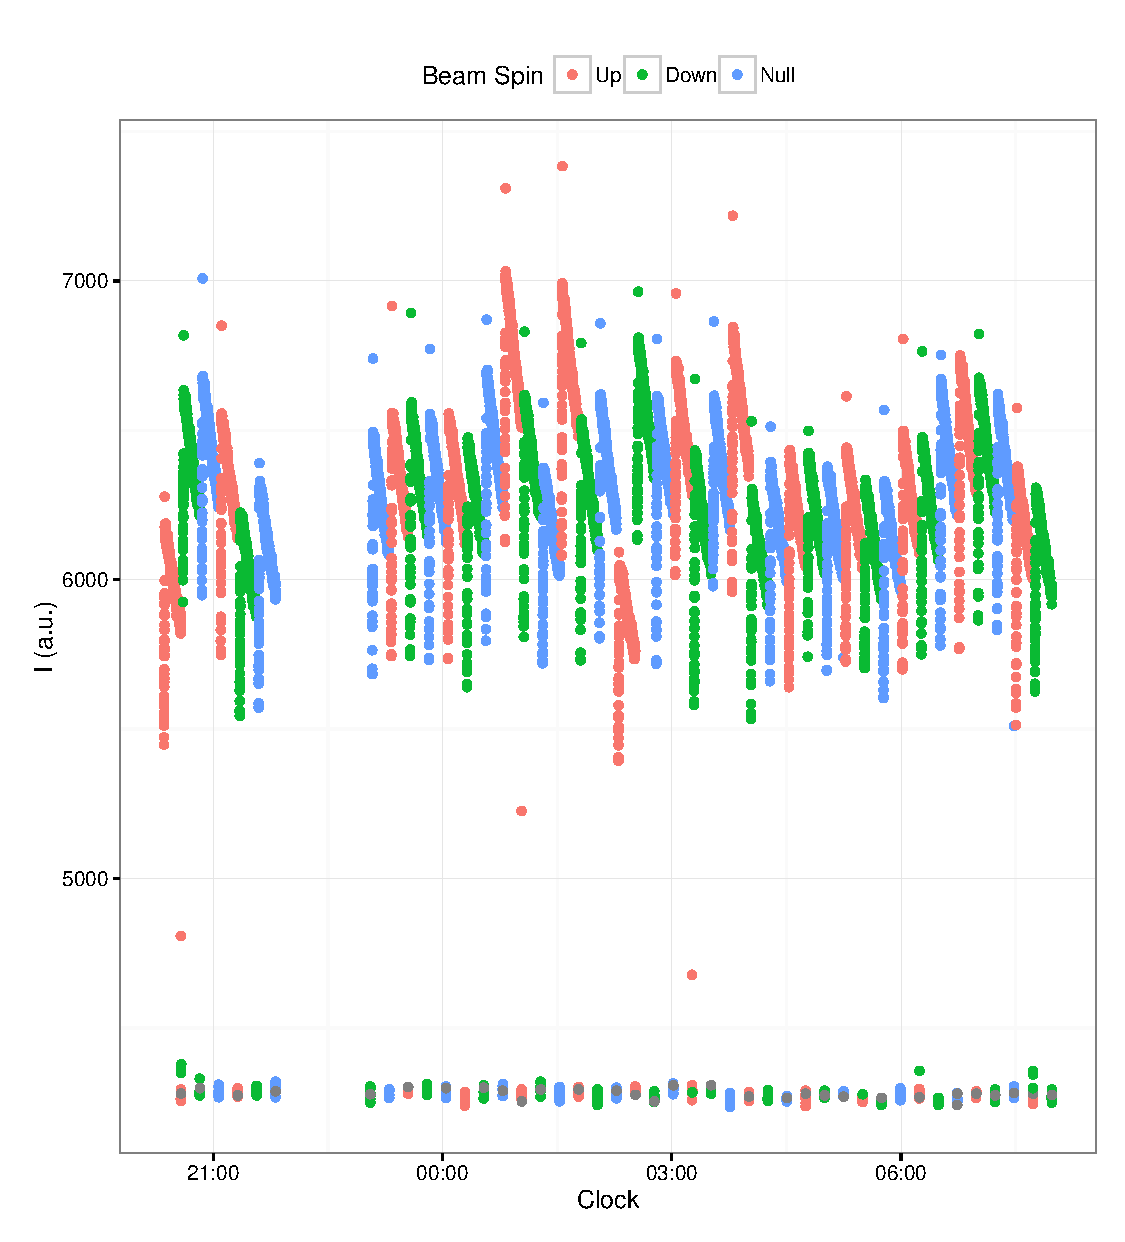
\includegraphics{Cycles2016.eps}
	\caption{Cycles in 2016 colored according to the beam spin state. Before 22:30 the target spin state is 3, after it is 1.\label{fig:Cycles}}
\end{figure}
\begin{figure}[H]
	\centering
	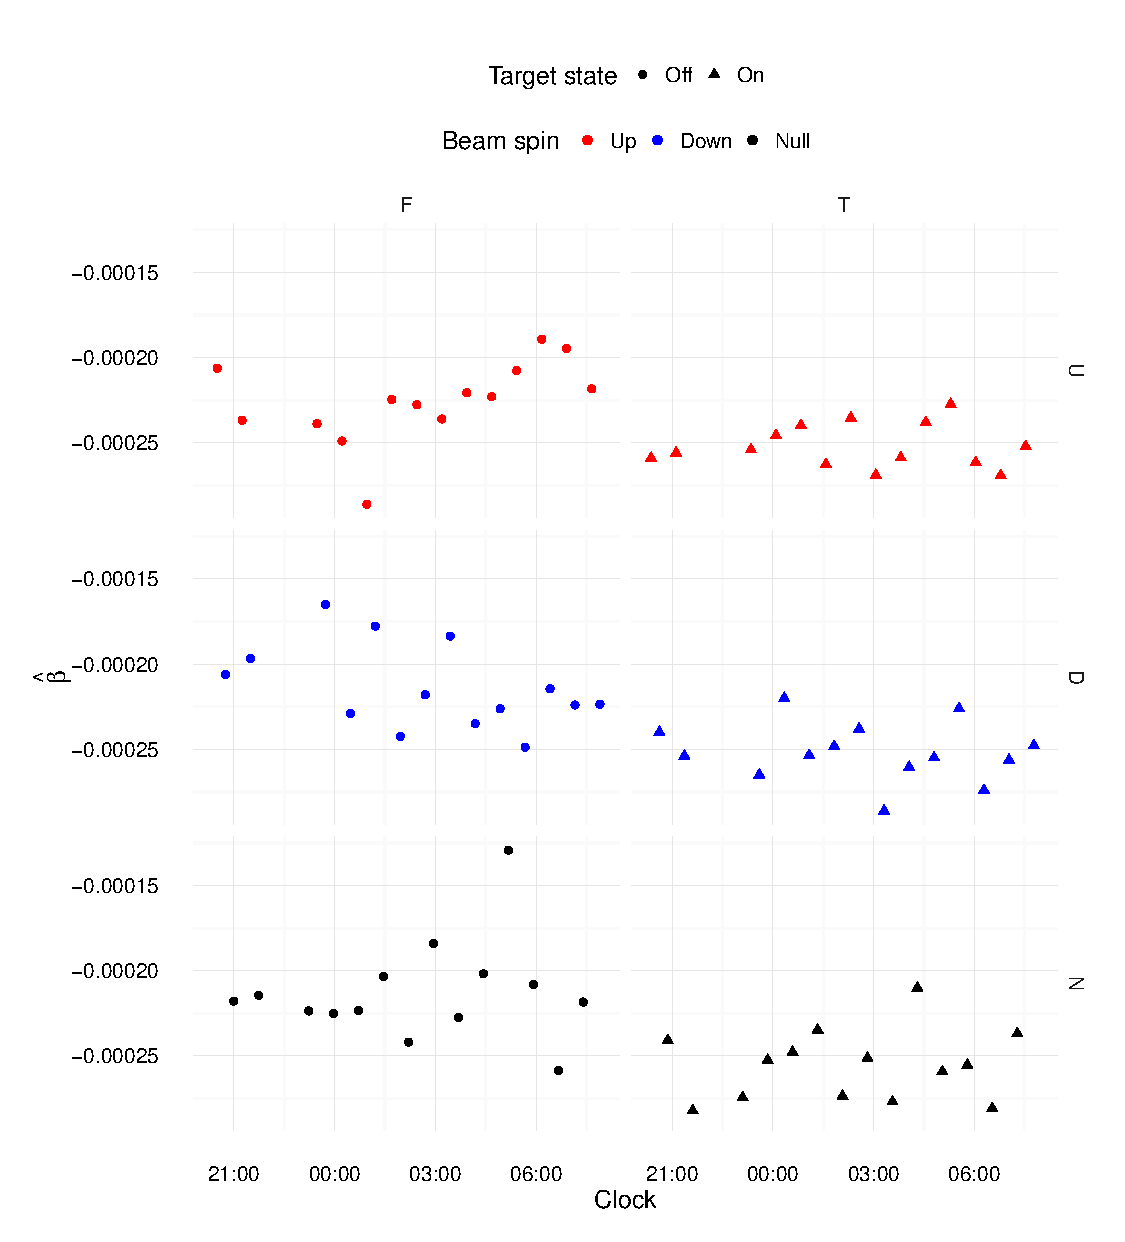
\includegraphics{Slopes2016_VS_Clock.eps}
	\caption{Slope estimates against time.\label{fig:Slopes}}
\end{figure}	
	
\newcommand{\vp}[2]{#1\cdot10^{#2}}
\begin{table}[h]
	\centering
	\caption{Slope summary statistics.\label{tbl:SlpSumStat}}
	\begin{tabular}{lllllrr}
		\hline\hline
		       Target        & Spin & \# & Mean (a.u.)      & SE (a.u.)    \\ \hline
		\multirow{3}{*}{Off} & Up   & 12 & $\vp{-2.26}{-4}$ & $\vp{7}{-6}$ \\
		                     & Down & 12 & $\vp{-2.16}{-4}$ & $\vp{8}{-6}$ \\
		                     & Null & 12 & $\vp{-2.12}{-4}$ & $\vp{9}{-6}$ \\ \hline
		\multirow{3}{*}{On}  & Up   & 12 & $\vp{-2.51}{-4}$ & $\vp{4}{-6}$ \\
		                     & Down & 12 & $\vp{-2.53}{-4}$ & $\vp{5}{-6}$ \\
		                     & Null & 12 & $\vp{-2.54}{-4}$ & $\vp{6}{-6}$ \\ \hline
	\end{tabular}
\end{table}


\section{Properties of the data}
The slopes summarized in Table~\ref{tbl:SlpSumStat} were obtained using Ordinary Least Squares regression. 
The Gauss-Markov theorem puts certain conditions on the data in order that the least squares slope estimator be minimum-variance mean-unbiased. Those conditions are:~\cite{GaussMarkov}
\begin{enumerate}
	\item Linearity and additivity of the relationship;
	\item Independence of the predictor and error variables (strict exogeneity);
	\item No serial correlation of the error;
	\item Constant variance of the error (homoskedasticity).
\end{enumerate}

The Breusch-Pagan test against heteroskedasticity suggests that our data are homoskedastic; however, the Durbin-Watson test for autocorrelation of the residuals (whose statistic is the value of the auto-correlation function at lag 1) yields the lag-1 autocorrelation around 60\% for all cycles (see Figure~\ref{fig:DW2}).~\footnote{The use of the generalized least squares model with the AR1-correlated error term did not improve the fit according to both the Akaike's and Bayesian information criteria.} Autocorrelation does not affect the slope estimate itself, but in its presence the OLS estimate of its standard error is biased. To correct for that, we use a robust standard error estimator provided by the \emph{sandwich} package of R.~\cite{RSandwich} The robust estimator takes care of both the (possible) heteroskedasticity, and the autocorrelation. 

\begin{figure}[H]
	\centering
	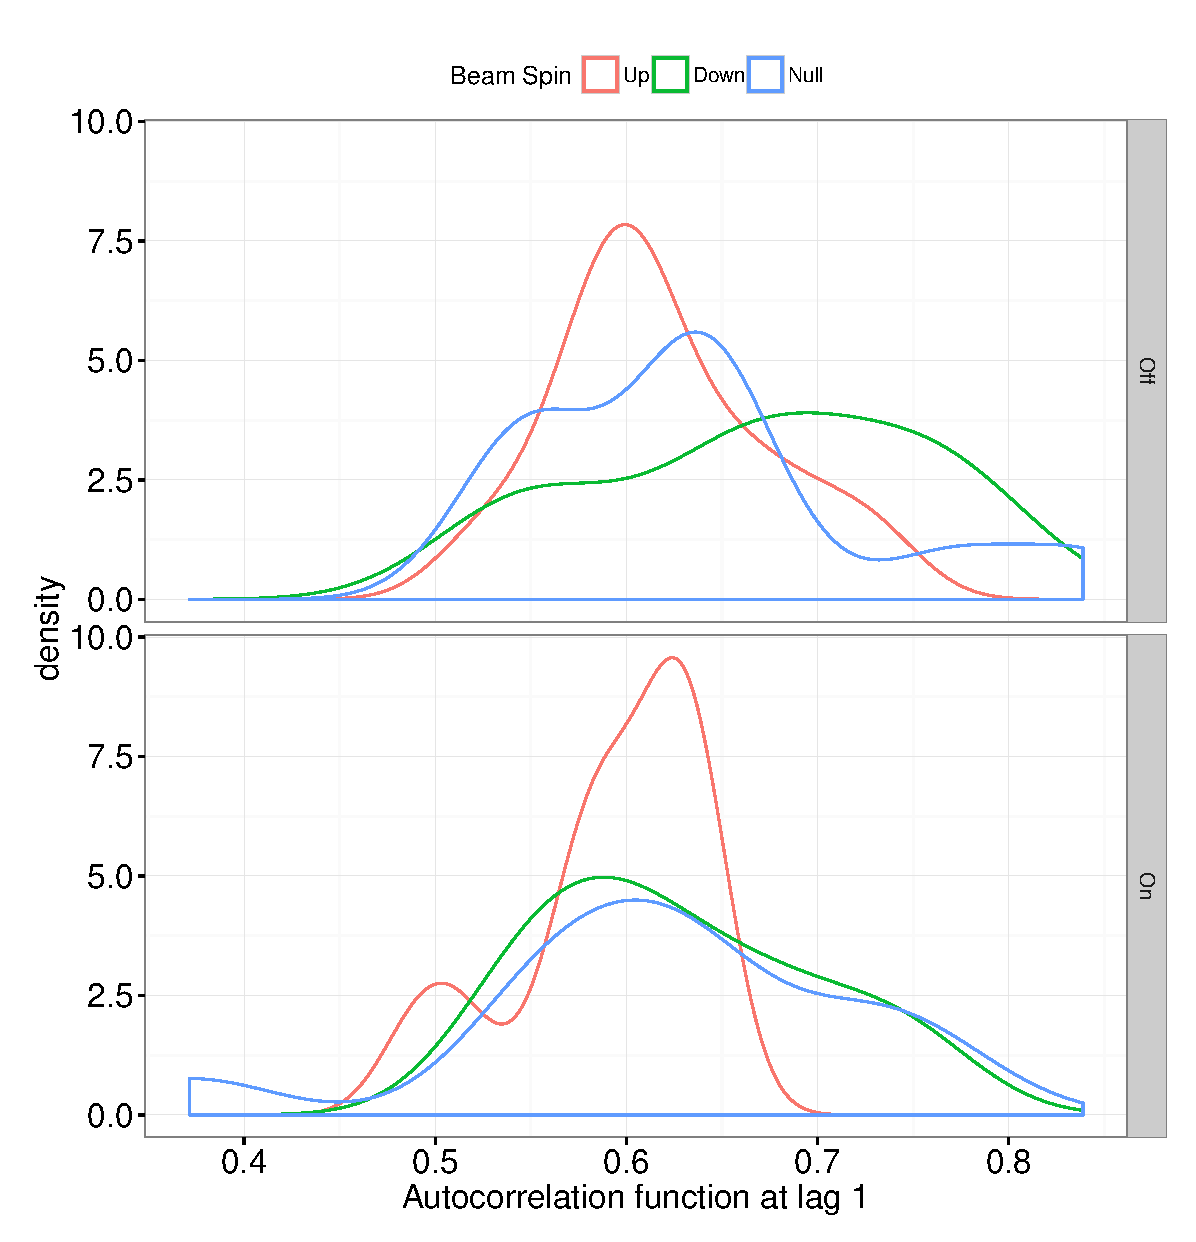
\includegraphics{ACF1_dens.eps}
	\caption{The distribution of the auto-correlation of the residuals at lag 1.\label{fig:DW2}}
\end{figure}

The moving Chow test, as well as other structural tests from the package~\cite{RStrucchange} suggest changes in the slope, i.e. the appropriateness of a piece-wise linear regression. The distribution of the breakpoints, as found by the Chow test, are plotted in Figure~\ref{FStat_BP_dens}. One can also observe from the plot of model residuals against the fitted values (Figure~\ref{fig:RvF-u17}) that the simple linear model is not appropriate for the data.

\begin{figure}[H]
	\centering
	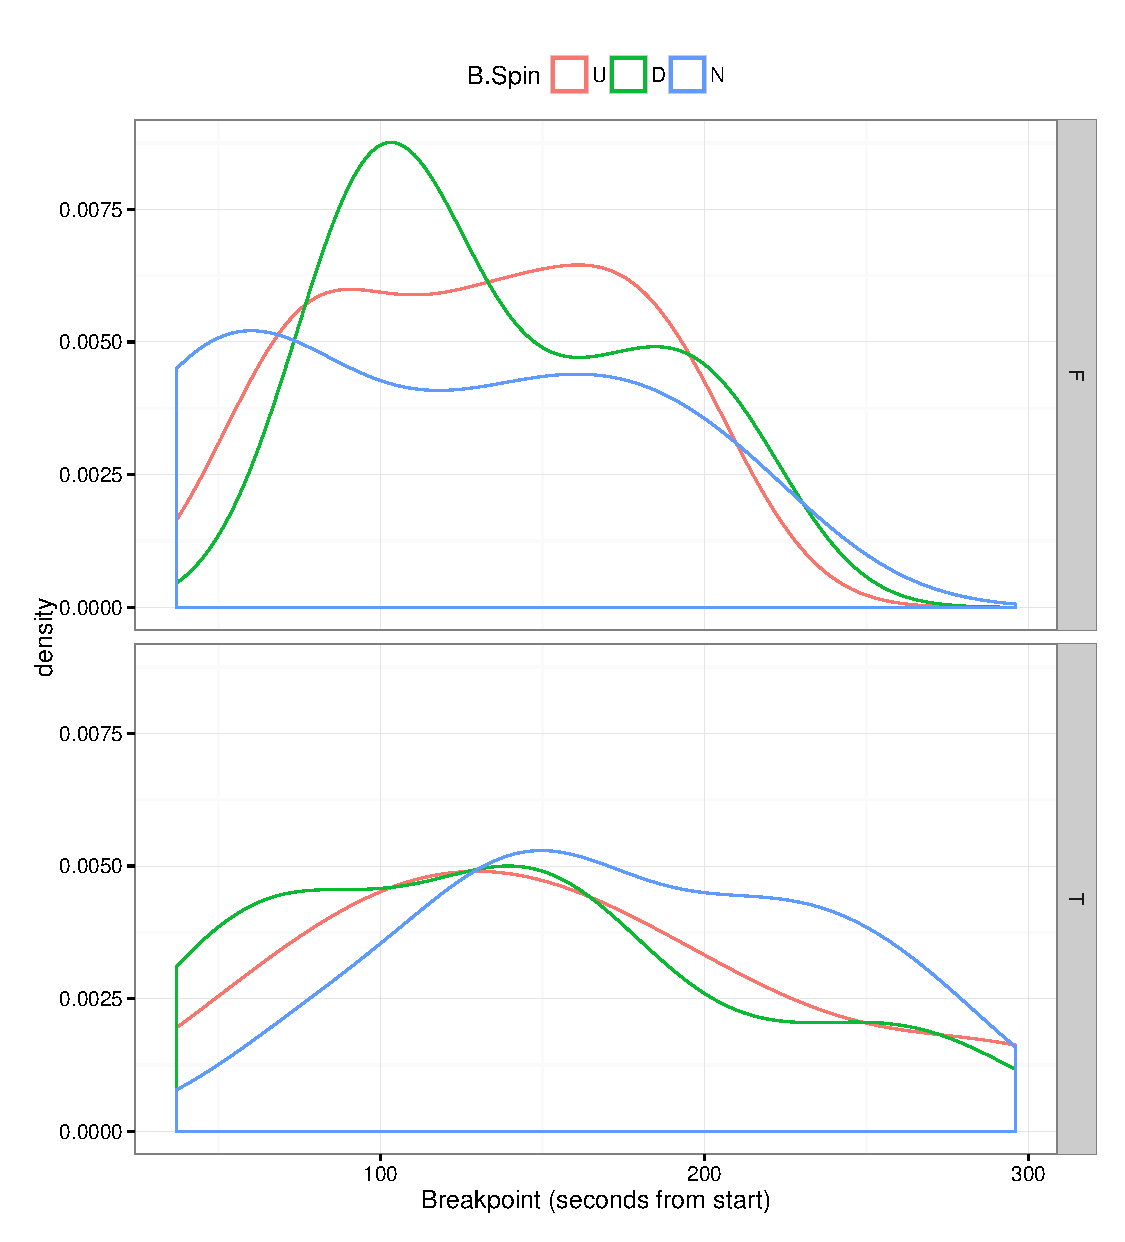
\includegraphics{FStats_BP_dens.eps}
	\caption{Point of change in the slope as found by the moving Chow test. The target-less cycles' distribution is in the upper panel.\label{FStat_BP_dens}}
\end{figure}

%\begin{figure}[H]
%	\centering
%	\begin{subfigure}{\textwidth}
%		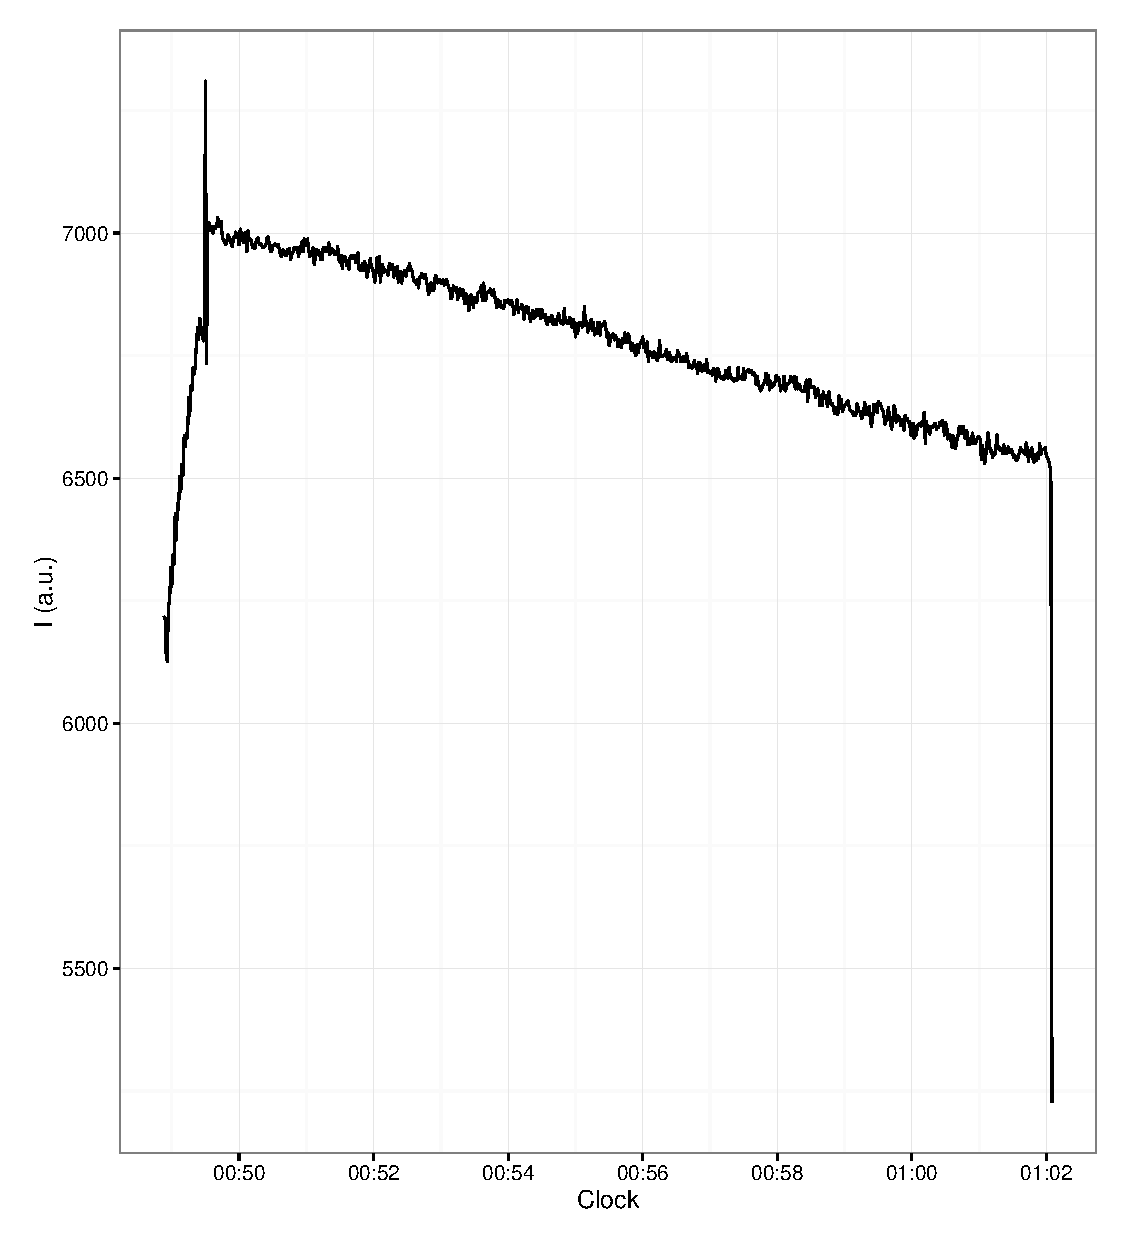
\includegraphics[height=.5\textheight]{TestCycle_2016-17.eps}
%		\caption{Example cycle.\label{fig:fig:TestCycle}}
%	\end{subfigure}
	\begin{figure}[H]
		\centering
		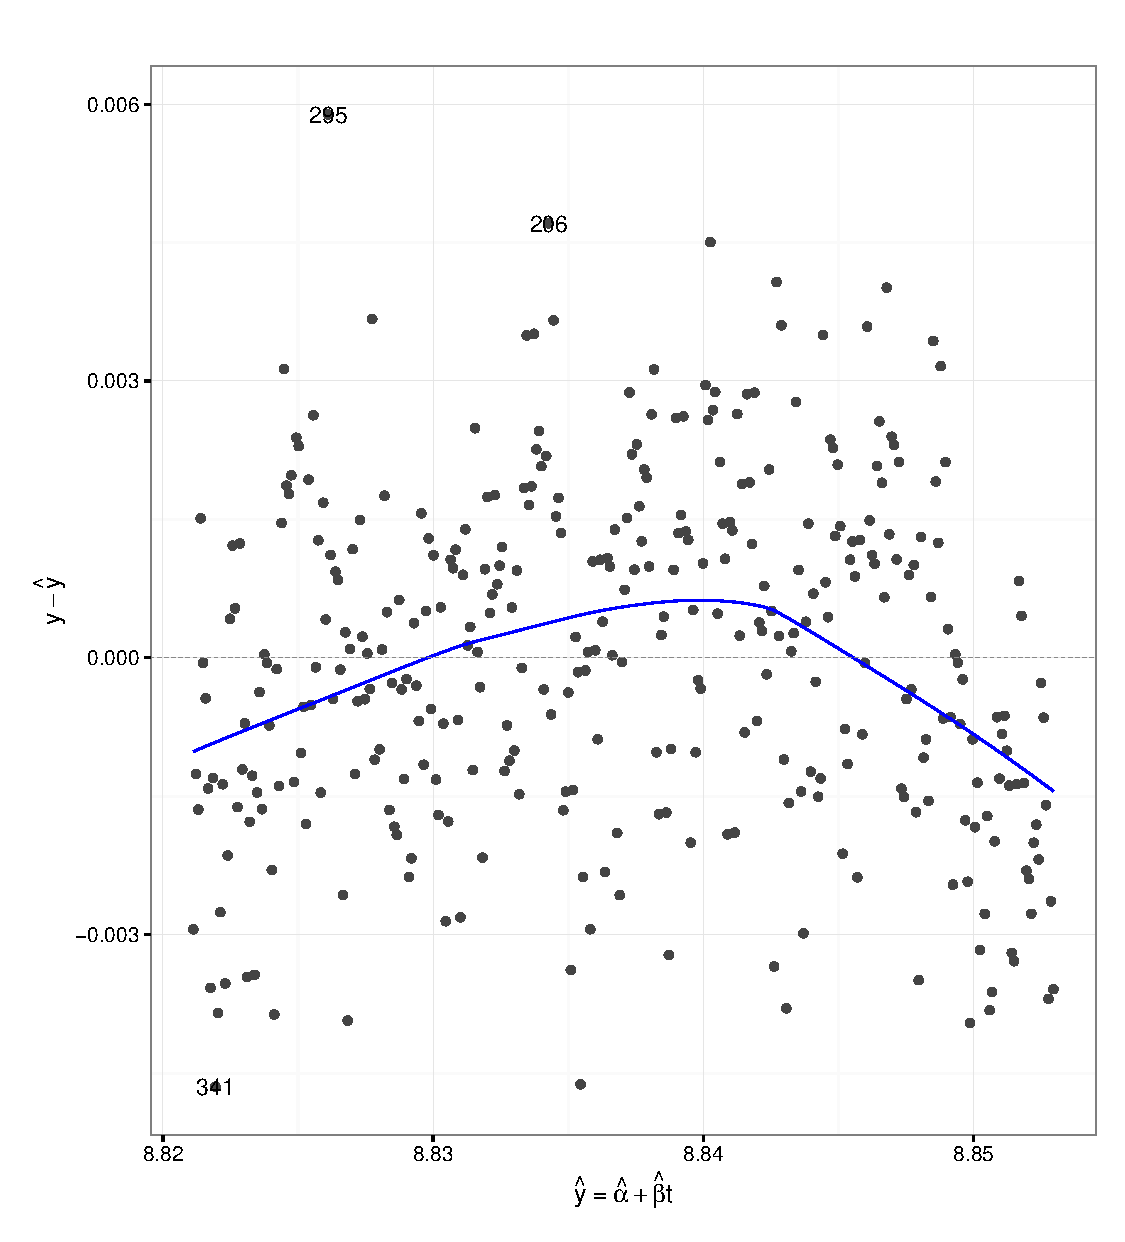
\includegraphics{Res_VS_Fit_2016-17.eps}
		\caption{Plot of the linear model residuals vs. the fitted values. The shape of the plot (flipped-over U) indicates that the model systematically overestimates the beam current at higher values, then underestimates in the mid range, and overestimates again at lower values.\label{fig:RvF-u17}}
	\end{figure}
%\end{figure}


Figure~\ref{fig:Slp_VS_I0} shows that there is a dependency between the beam's life time and its intensity. The initial beam intensity $I_0$ was estimated as the exponentiated intercept of the linear model $\ln I_t = \ln I_0 + \slp\cdot t + \err_t$, and the life time estimate is $\hat{\tau} = -\sfrac{1}{\slp*}$. 

\begin{figure}[H]
	\centering
	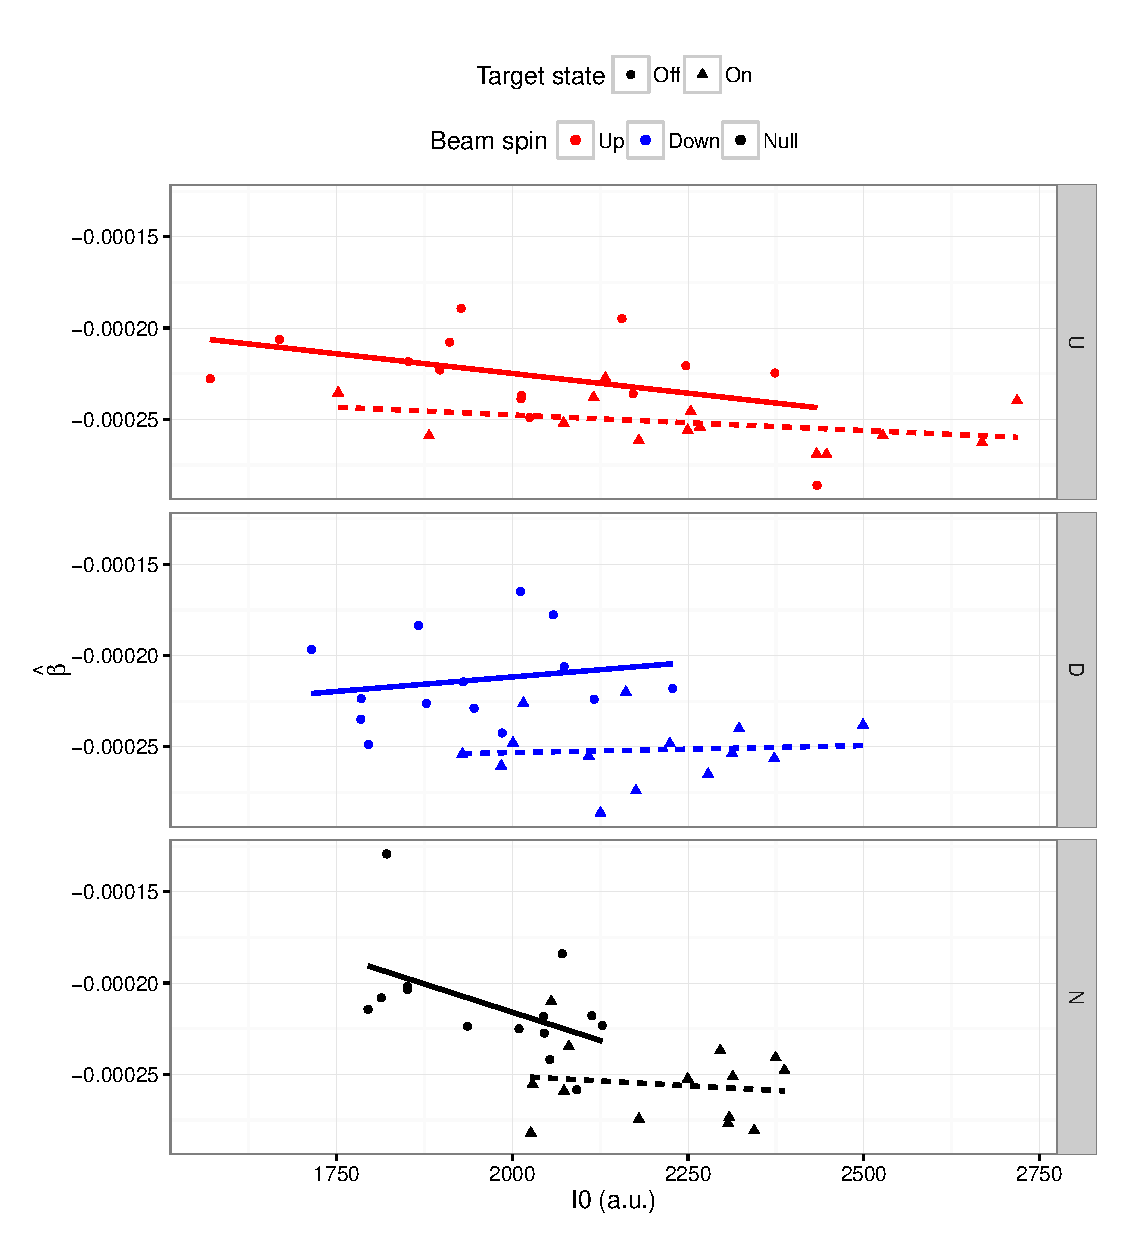
\includegraphics{Slope_VS_IniCurrent_2016.eps}
	\caption{Slope estimates against the initial beam current. The beam current is estimated from the regression model.\label{fig:Slp_VS_I0}}
\end{figure}

\section{Obtainable estimates}

The slopes we estimate are presumed to have the following, most general, form:
\begin{equation}
	\slp = -\nu\bkt*{\CS[0]\bkt{1 + \Ayy P^t_y P_y}\Thick + \CS[X]\Thick[X]},
\end{equation}
where $nu$ is the beam revolution frequency, $\CS[0]$ is the unpolarized cross section, $\Ayy$ is the asymmetry, $P^t_y$ and $P_y$ are the vertical components of respectively the target and beam polarization vectors, $\Thick = \rho d$ [cm$^{-2}$] is the target thickness, and $\CS[X]\Thick[X]$ refers to the extra-target loss.

In principle, we can estimate both the unpolarized cross section and the asymmetry from the data we have. If we take the difference between two null beam spin state slopes ($P_y = 0$),~\footnote{This is done in order to remove the dependency on the unknown value of $\Ayy$.} one from a target-off cycle, the other target-on, 
\[
	\slp[off]^0 - \slp[on]^0 = \nu\CS[0]\bkt{\Thick[on]-\Thick[off]},
\]
from which we can estimate $\CS[0]$, once we know the target thicknesses.

The asymmetry is estimated by taking the difference between two target-on slopes with opposite beam polarizations as in
\[
	\slp[on]^- - \slp[on]^+ = \nu\CS[0]\Thick[on] P^t\DP*\Ayy.
\]
\subsection{Cross section}
We used the thicknesses estimated from the shift of the Schottky spectrum~\cite{Stein} ($\Thick[on] = \vp{1.1}{14}$ [cm$^{-2}$], and $\Thick[off] = 0$ [cm$^{-2}$]). The cross section estimates we got are presented in Figure~\ref{fig:CS0au_dens} and Table~\ref{tbl:CS0SumStat}. Those estimates that are based on slopes that are considered outliers according to Tukey's range test are labeled unsound, and those whose slopes are separated by more that 40 minutes are considered far removed. The latter classification was introduced in connection with the concern that the environmental conditions systematically changed over time.

\begin{figure}[H]
	\centering
	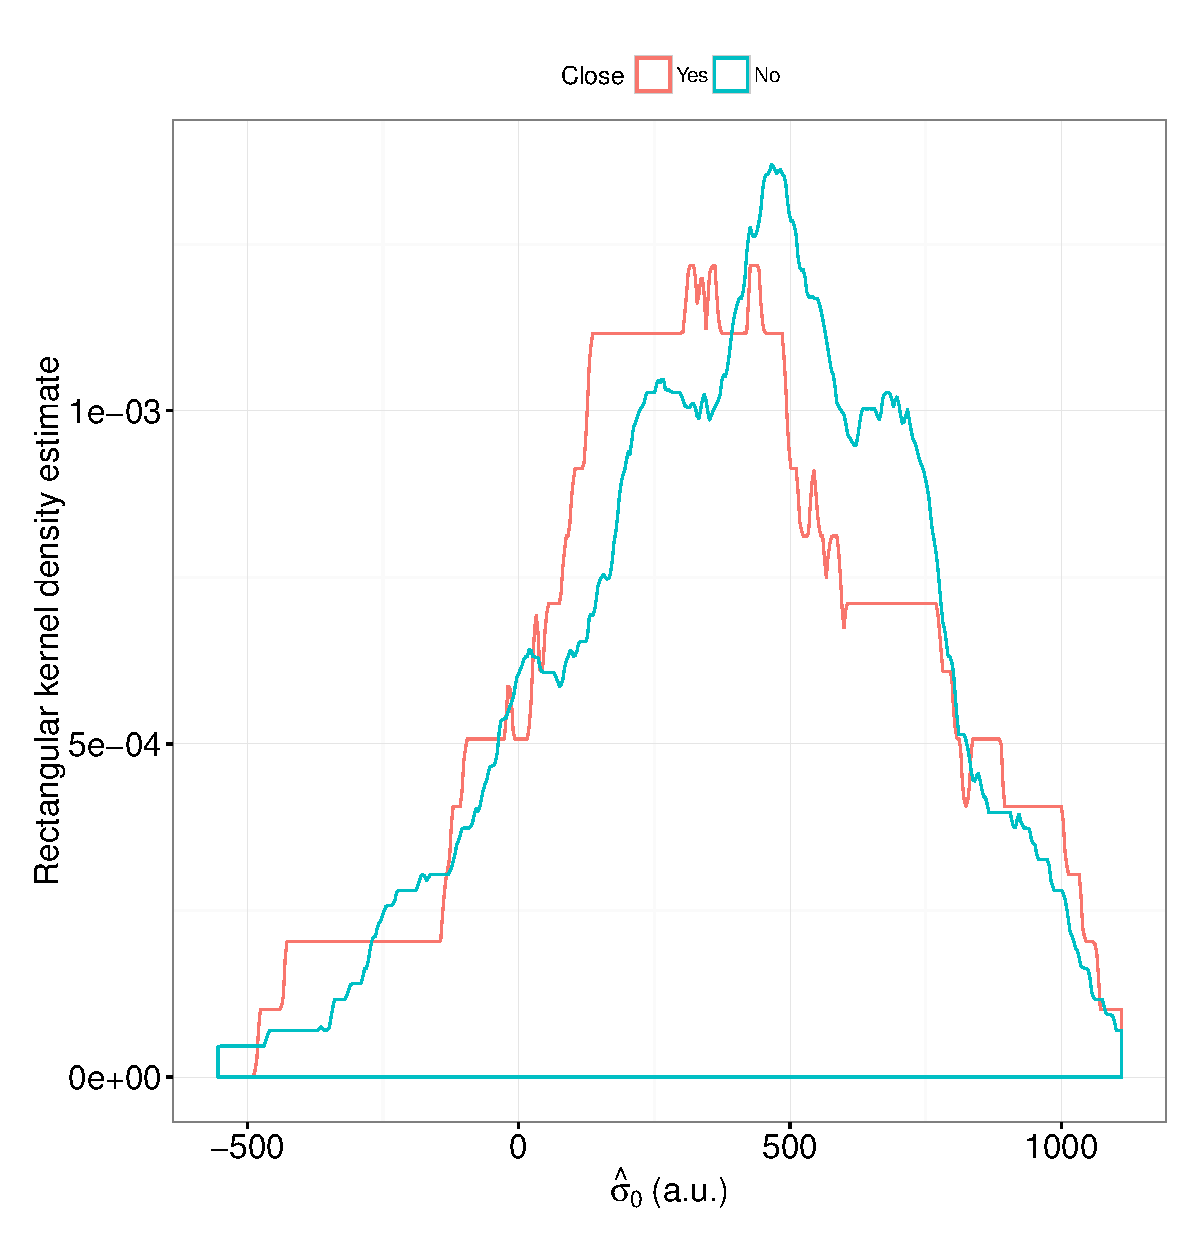
\includegraphics{CS0_au_dens.eps}
	\caption{Rectangular kernel density estimate of cross section.\label{fig:CS0au_dens}}
\end{figure}

\begin{threeparttable}[H]
	\centering
	\caption{Cross section summary statistics\label{tbl:CS0SumStat}}
	\begin{tabular}{llrrrrrr}
		\hline\hline
		Sound                & Close &  \# & Mean\tnote{a} (a.u.) & SE\tnote{b} (a.u.) & $\chi^2_{red}$ & SE\tnote{c} (a.u.) &  Mode\tnote{d} (a.u.)\\ \hline
		\multirow{3}{*}{Yes} & Yes   &  21 &                  366 &                 73 &            6.5 &                178 &  386 \\
		                     & No    & 111 &                  397 &                 30 &            7.0 &                 80 &  403 \\
		                     & All   & 132 &                  393 &                 28 &            6.9 &                 73 &  400 \\ \hline
		\multirow{3}{*}{No}  & Yes   &   2 &                 1469 &                 22 &            0.1 &                  5 & 1467 \\
		                     & No    &  10 &                 1440 &                 83 &            4.2 &                169 & 1429 \\
		                     & All   &  12 &                 1444 &                 69 &            3.4 &                127 & 1435 \\ \hline
	\end{tabular}
	\begin{tablenotes}
		\item[a]{Variance weighted mean.}
		\item[b]{The distribution's standard deviation divided by the square root of the sample size.}
		\item[c]{According to the formula, correcting for dispersion via the $\chi^2_{red}$.}
		\item[d]{Most frequent value.}
	\end{tablenotes}
\end{threeparttable}

\subsection{Asymmetry}

The summary statistics for the asymmetry are presented in Table~\ref{tbl:AyySumStat}; its density estimate in Figure~

\begin{threeparttable}[H]
	\centering
	\caption{Asymmetry summary statistics\label{tbl:AyySumStat}}
	\begin{tabular}{llrrrrrlr}
		\hline\hline
		Sound                & Close &  \# & $\CS*[0]$ (a.u.) & Mean\tnote{a} (a.u.) & SE\tnote{b} (a.u.) & $\chi^2_{red}$ & SE\tnote{c} (a.u.) & Mode\tnote{d} (a.u.) \\ \hline
		\multirow{3}{*}{Yes} & Yes   &  23 &              366 &       $\vp{2.0}{-2}$ &     $\vp{9.1}{-2}$ &            5.8 & 0.23               &      $\vp{-4.2}{-2}$ \\
		                     & No    & 121 &              397 &       $\vp{2.2}{-2}$ &     $\vp{4.6}{-2}$ &            8.2 & 0.13               &      $\vp{-3.0}{-2}$ \\
		                     & All   & 144 &               -- &       $\vp{2.2}{-2}$ &     $\vp{4.2}{-2}$ &            7.8 & 0.12               &      $\vp{-3.1}{-2}$ \\ \hline
	\end{tabular}
	\begin{tablenotes}
		\item[a]{Variance weighted mean.}
		\item[b]{The distribution's standard deviation divided by the square root of the sample size.}
		\item[c]{According to the formula, correcting for dispersion via the $\chi^2_{red}$.}
		\item[d]{Most frequent value.}
	\end{tablenotes}
\end{threeparttable}

\begin{figure}
	\centering
	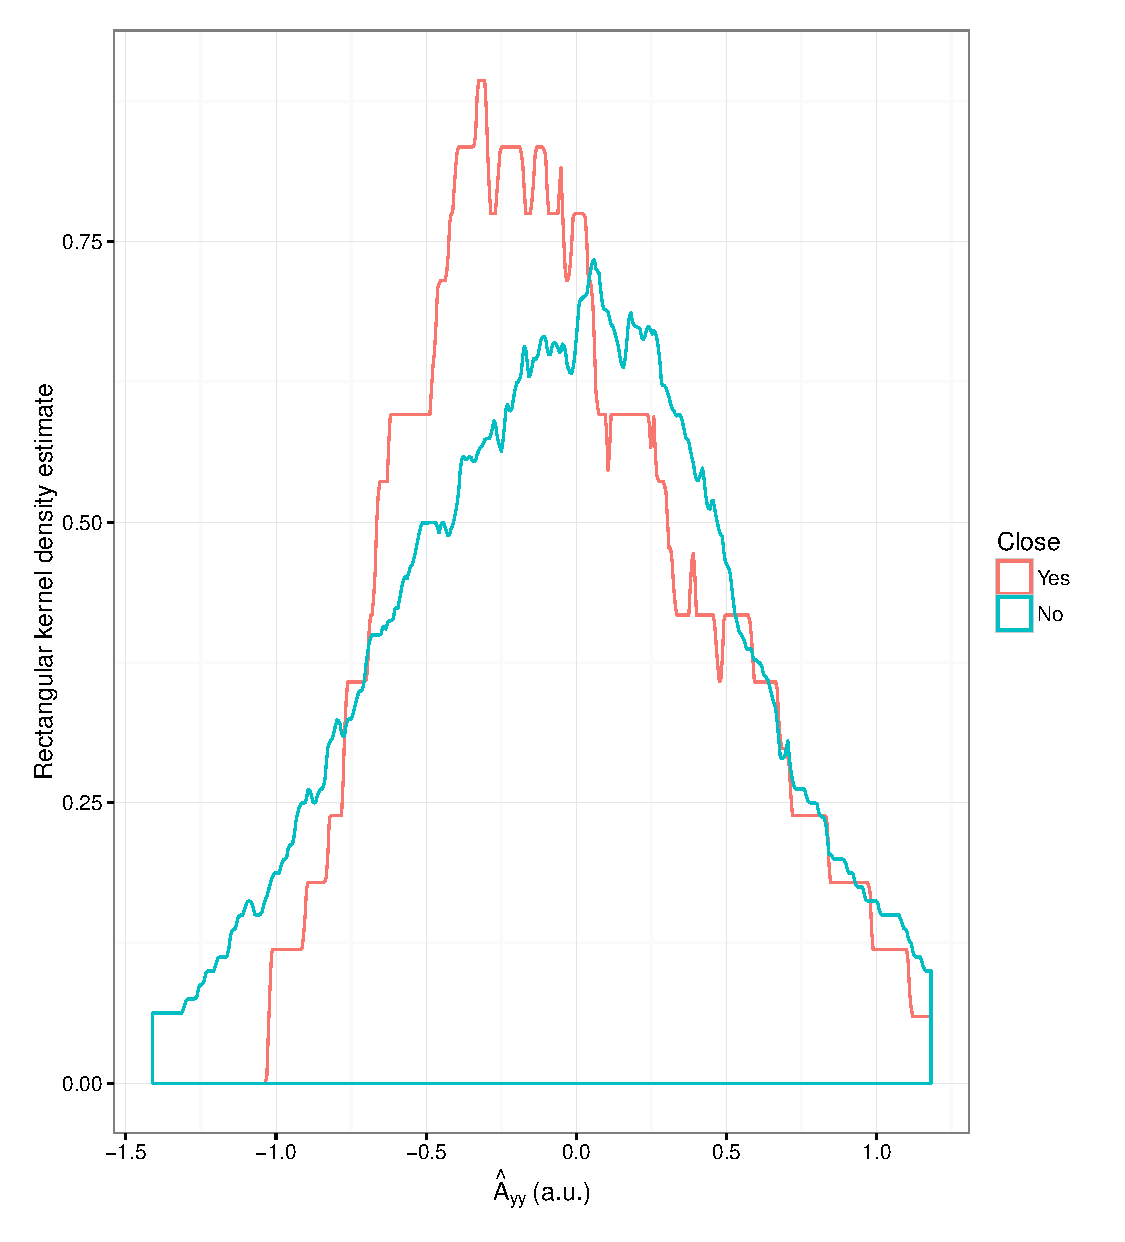
\includegraphics{Ayy_dens.eps}
	\caption{Kernel density estimate of $\Ayy$.}
\end{figure}

\begin{thebibliography}{9}
	\bibitem{GaussMarkov}
	D.S.G. Pollock. ``Topics in Econometrics.''
	\bibitem{RSandwich}
	\url{https://cran.r-project.org/web/packages/sandwich/sandwich.pdf}
	\bibitem{RStrucchange}
	\url{https://cran.r-project.org/web/packages/strucchange/strucchange.pdf}
	\bibitem{Stein}
	H. J. Stein, M. Hartmann, I. Keshelashvili, et al. ``Determination of target thickness and luminosity from beam energy losses.''
\end{thebibliography}

\end{document}